\section{Dashboard} \label{dash}
\begin{figure}[H]
\centering
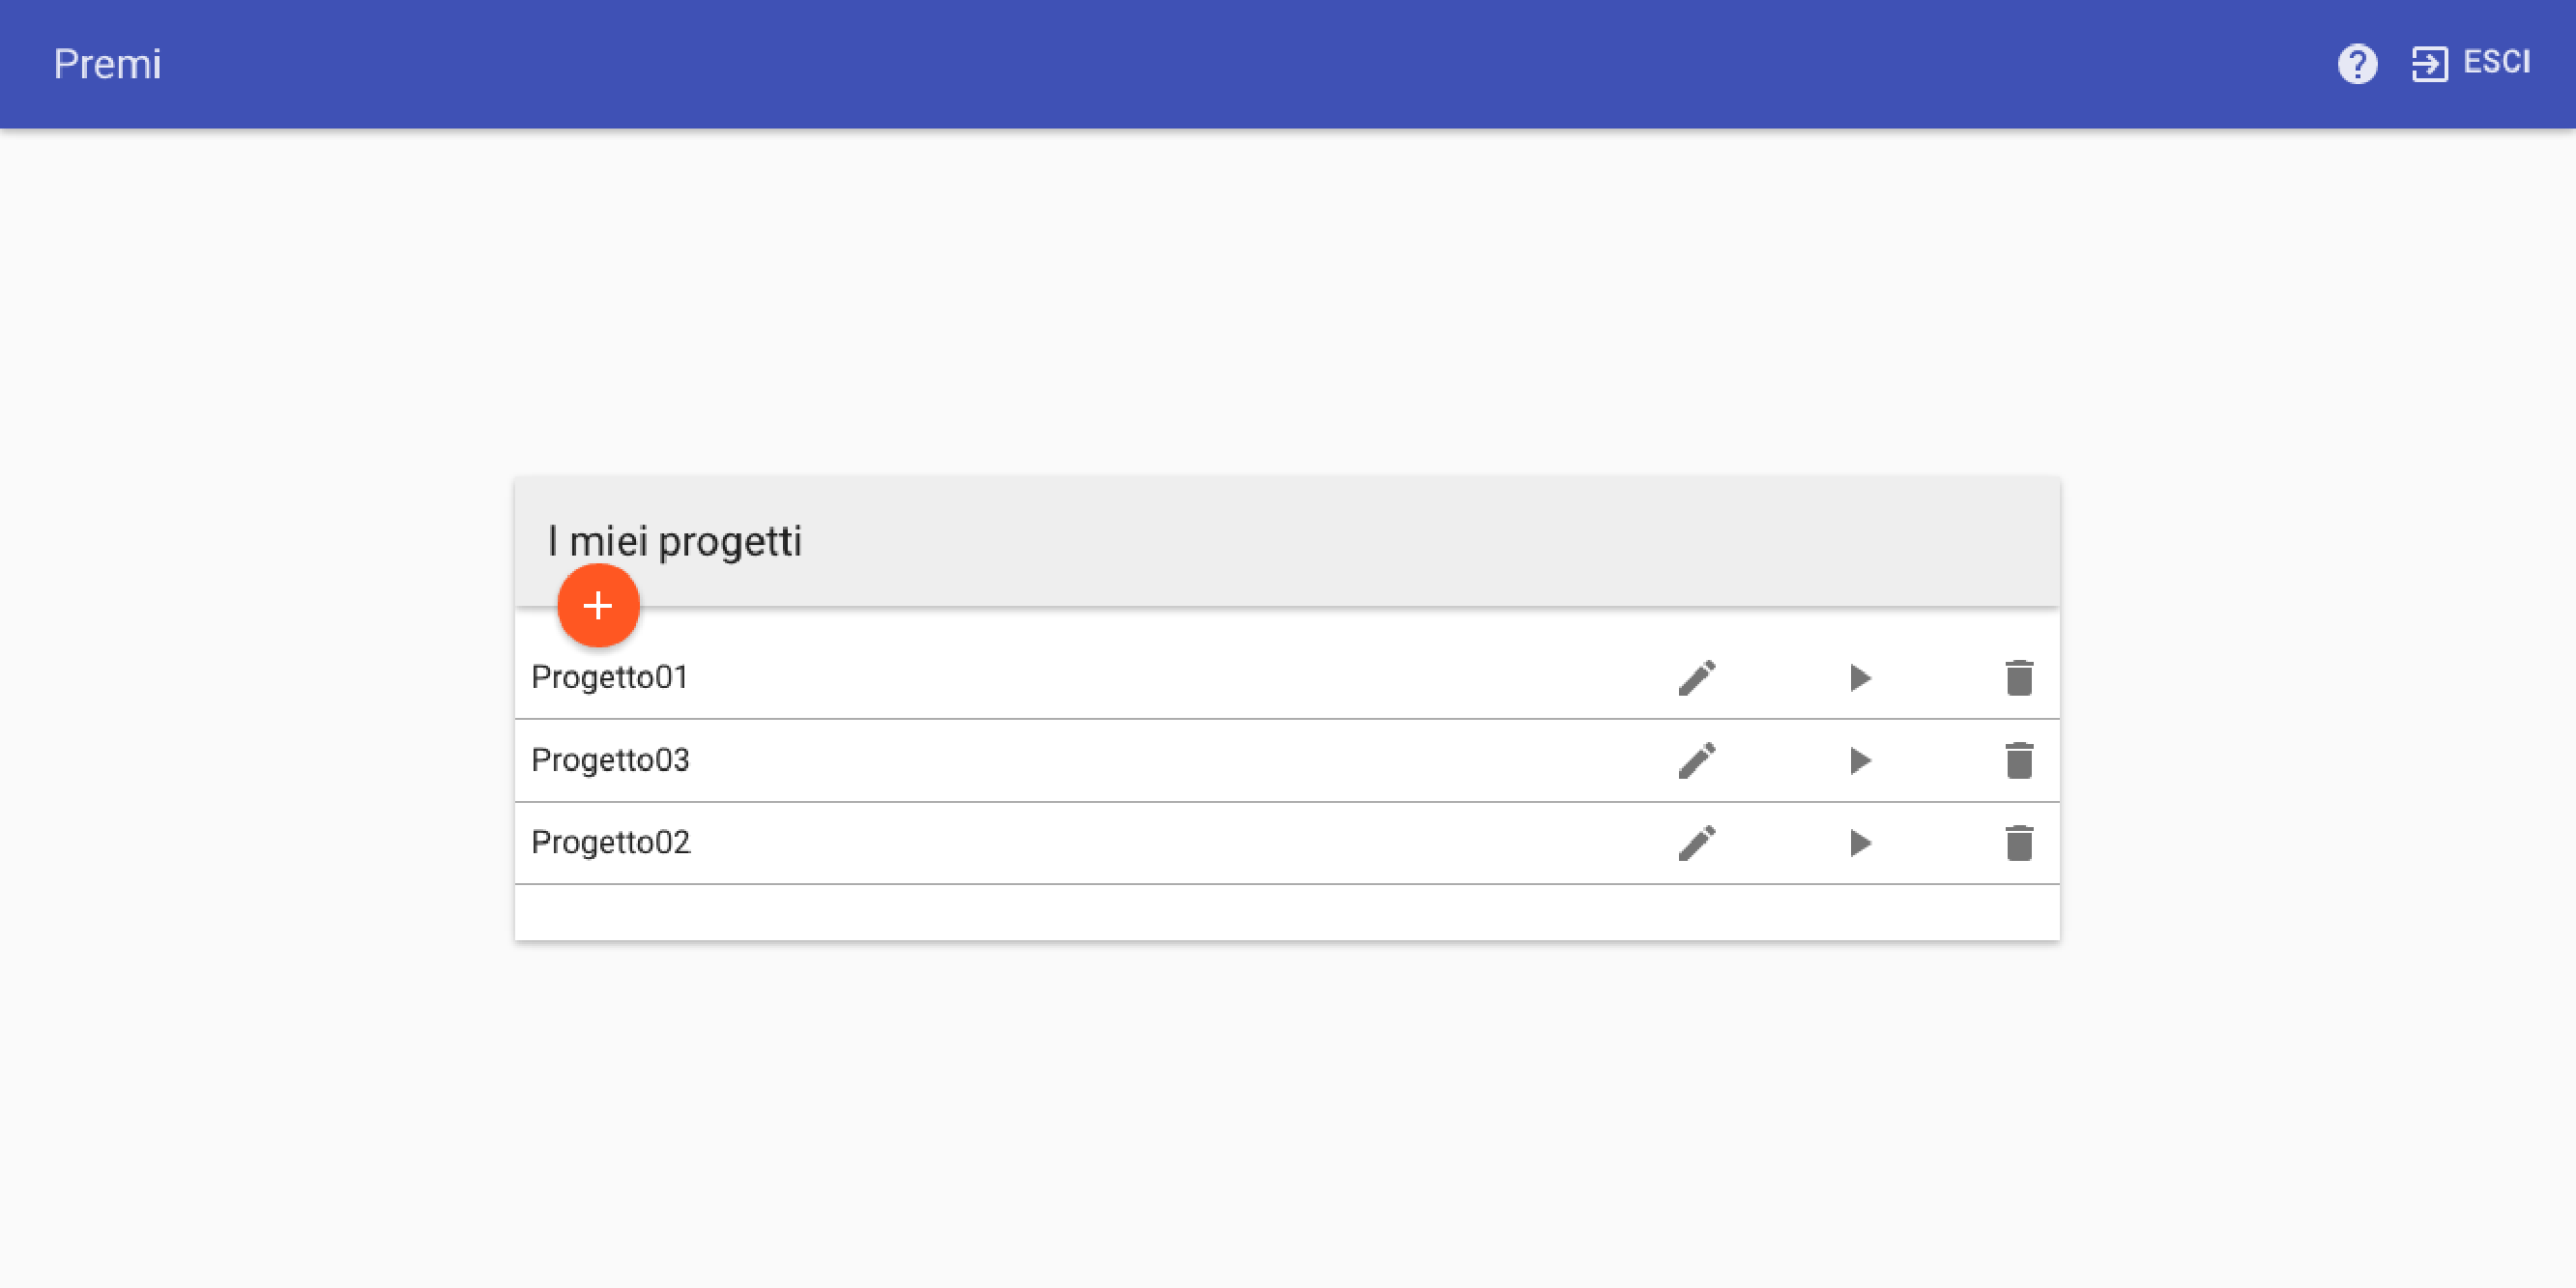
\includegraphics[scale=0.3]{immagini/dashboard.pdf}
\caption{Dashboard}
\end{figure}
In seguito all'autenticazione o alla registrazione l'utente verrà reindirizzato alla \textit{Dashboard}.\\
La \textit{Dashboard} presenta una finestra che contiene al suo interno la lista dei \gloxy{progetti} personali dell'utente. Per ogni \gloxy{progetto}, all'interno della lista, sono presenti dei pulsanti che permettono di eseguite varie azioni sul rispettivo \gloxy{progetto}.
Mediante i pulsanti presenti nella lista dei \gloxy{progetti} l'utente può crearne di nuovi, eliminare dei \gloxy{progetti} già esistenti oppure può modificare o effettuare una presentazione di un determinato \gloxy{progetto}. \\
\begin{figure}[H]
\centering
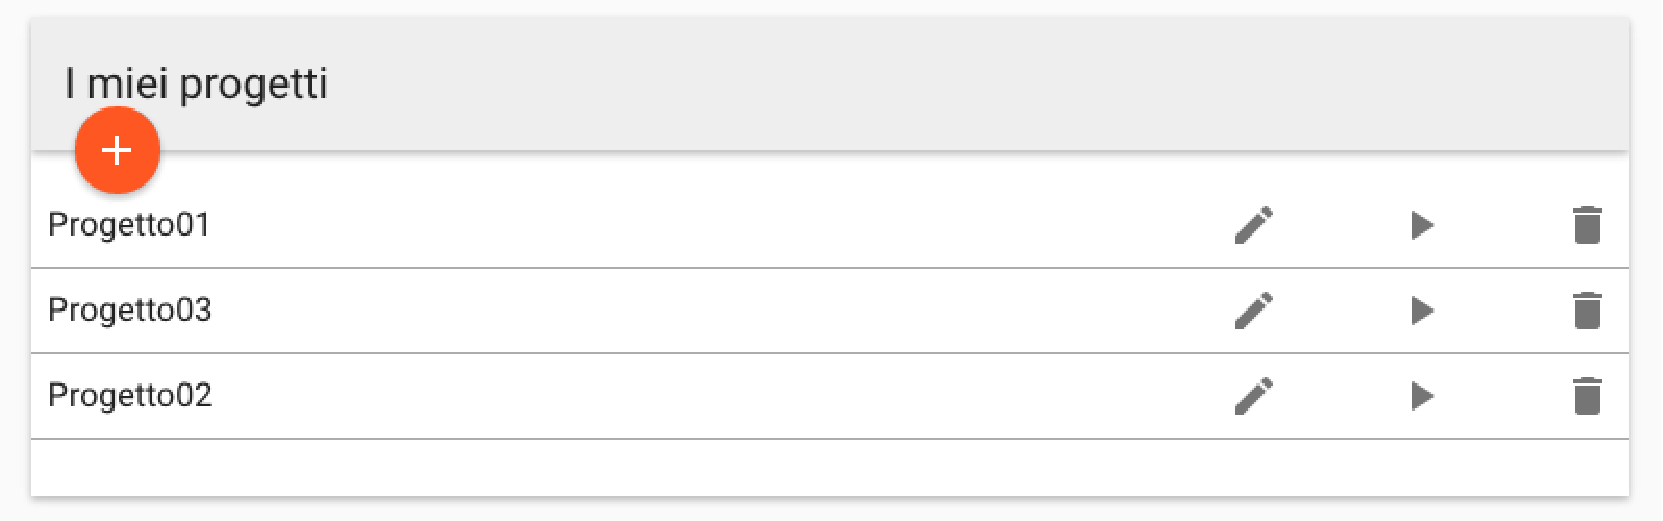
\includegraphics[scale=0.5]{immagini/dashboardVuota.pdf}
\caption{Dashboard - lista dei progetti}
\end{figure}
\subsection{Creazione nuovo progetto}
L'utente può creare un nuovo progetto premendo il pulsante \textbf{più} 
\includegraphics[scale=0.5]{immagini/piuButton.pdf} che si trova nella parte alta della finestra contenente la lista progetti.\\
Effettuando questa azione verrà aggiunto il nuovo progetto alla lista progetti.
\begin{figure}[H]
\centering
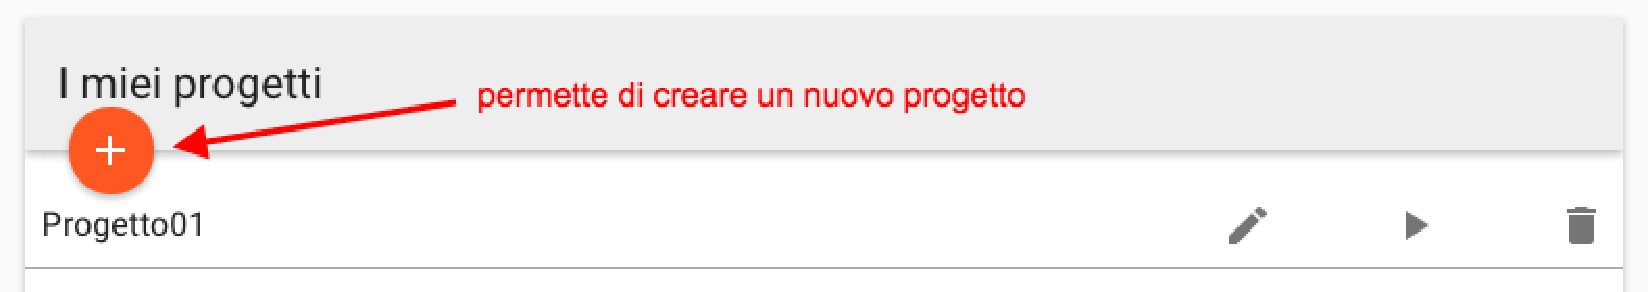
\includegraphics[scale=0.5]{immagini/imgCreaProg.pdf}
\caption{Dashboard - crea nuovo progetto}
\end{figure}
\subsection{Eliminazione di un progetto}
Per poter eliminare un progetto l'utente dovrà premere il pulsante contenente l'icona rappresentante un cestino, che si trova nella riga relativa al progetto che desidera eliminare e confermare l'operazione.
\begin{figure}[H]
\centering
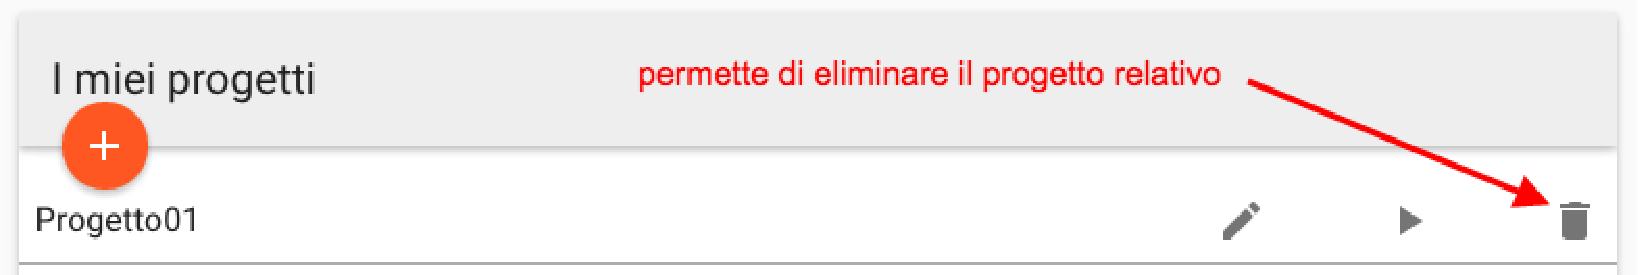
\includegraphics[scale=0.5]{immagini/imgEliminaProg.pdf}
\caption{Dashboard - elimina progetto}
\end{figure}
\subsection{Modificare un progetto}
Per poter accedere alla modalità di editing del progetto l'utente dovrà premere il pulsante contenente l'icona rappresentante una matita, che si trova nella riga relativa al progetto che si desidera modificare.
\begin{figure}[H]
\centering
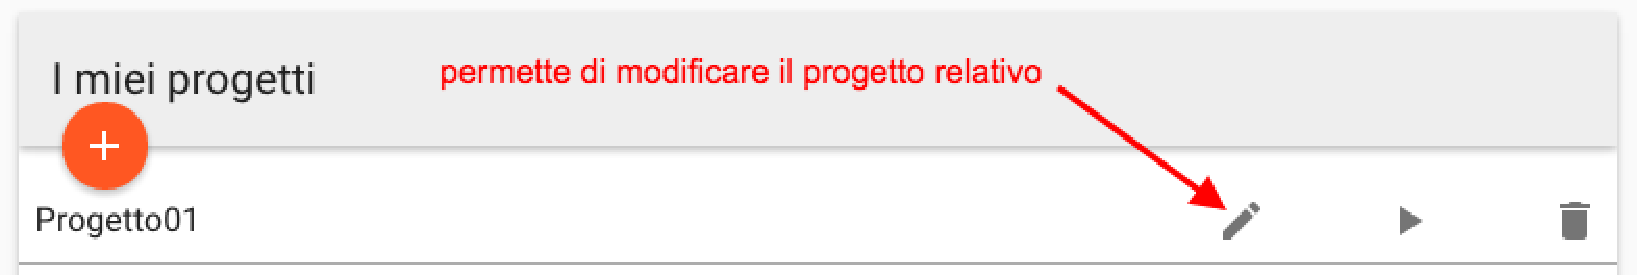
\includegraphics[scale=0.5]{immagini/imgModificaProg.pdf}
\caption{Dashboard - modifica progetto}
\end{figure}
\subsection{Avviare la presentazione di un progetto}
Per poter avviare la presentazione di un \gloxy{progetto}, l'utente deve premere il pulsante contenente l'icona rappresentante il simbolo \textit{play}, che si trova nella riga relativa al \gloxy{progetto} che si desidera presentare.\\ Successivamente, verrà visualizzata una nuova finestra nella quale l'utente dovrà selezionare il \gloxy{percorso} di presentazione e, una volta selezionato, verrà avviata la presentazione.
\begin{figure}[H]
\centering
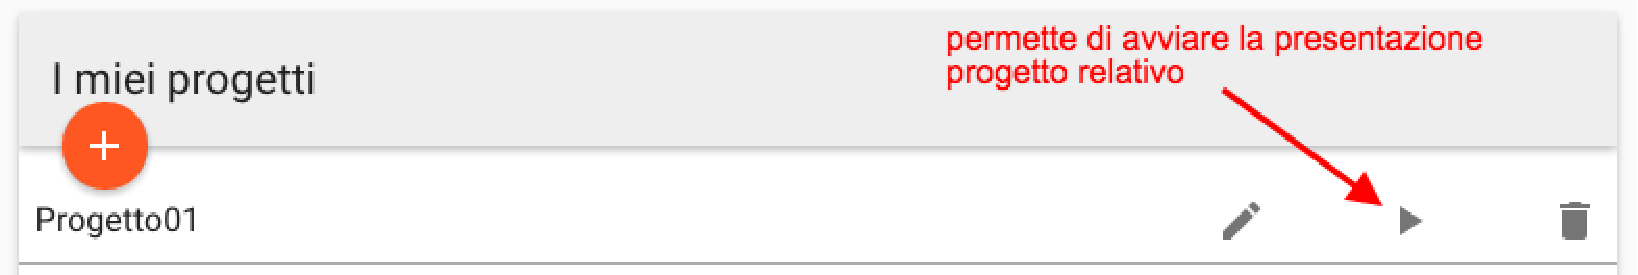
\includegraphics[scale=0.5]{immagini/imgPresentProg.pdf}
\caption{Dashboard - avviare la presentazione di un progetto}
\end{figure}
